\documentclass[a4paper, 12pt]{article}

\usepackage{multirow}
\usepackage[table,xcdraw]{xcolor}
\usepackage{enumerate}
\usepackage{graphicx}
\usepackage[T5]{fontenc}
\usepackage[utf8]{inputenc}
\usepackage[margin = 2cm]{geometry}
\usepackage{amsfonts, amsmath, amssymb}
\usepackage[none]{hyphenat}
\usepackage{fancyhdr}
\usepackage{float}
\usepackage{hyperref}
\usepackage{caption}
\usepackage[nottoc, notlot, notlof]{tocbibind}

\captionsetup[table]{skip=5pt}
\pagestyle{fancy}
\fancyhead[L]{Trường Đại học Khoa học Tự nhiên - ĐHQG TP.HCM}
\fancyhead[R]{Nhóm Just $4^{th}$}

\begin{document}

\begin{titlepage}
	\begin{center}
		\vspace*{1cm}
		\Large\textbf{Báo cáo \#3\\Giao diện người dùng \& Kiểm thử}\\

		\vfill
		\line(1,0){450}\\[4mm]
		\LARGE\textbf{\MakeUppercase{Dự án quản lý tạp chiếu phim}}\\[3mm]
		\Large{Nhập môn Công nghệ phần mềm (CSC13002)}\\[3mm]
		\Large{Nhóm Just $4^{th}$}
		\line(1,0){430}\\
		\vfill

		\vfill
		TP Hồ Chí Minh, ngày 09/12/2020
	\end{center}
\end{titlepage}

\tableofcontents
\thispagestyle{empty}
\clearpage

\section{Thông tin nhóm}
\label{sec:info}
\begin{enumerate}
	\item \textbf{Đường link GitHub}: \url{https://github.com/baolongnguyenmac/CinemaManagementSystem}
	\item \textbf{Đường link Trello}: \url{https://trello.com/b/OmRBLunD/báo-cáo-giao-diện-kiểm-thử}
	\item \textbf{Danh sách thành viên}
	\begin{table}[H]
		\begin{center}
			\begin{tabular}{|c|c|l|c|c|}
				\hline
				STT & MSSV     & \multicolumn{1}{c|}{Họ tên} & Email                         & SĐT        \\ \hline
				1   & 18120201 & Nguyễn Bảo Long             & 18120201@student.hcmus.edu.vn & 0919070940 \\ \hline
				2   & 18120211 & Võ Thế Minh                 & 18120211@student.hcmus.edu.vn & 0981850699 \\ \hline
				3   & 18120227 & Phạm Văn Minh Phương        & 18120227@student.hcmus.edu.vn & 0343049359 \\ \hline
				4   & 18120210 & Phạm Tống Bình Minh         & 18120210@student.hcmus.edu.vn & 0971877781 \\ \hline
				5   & 18120264 & Nguyễn Duy Vũ               & 18120264@student.hcmus.edu.vn & 0911572108 \\ \hline
			\end{tabular}
			\caption{Bảng danh sách thành viên nhóm}
		\end{center}
	\end{table}
\end{enumerate}
\clearpage

\section{Lịch sử cập nhật}
\label{sec:history}
\begin{table}[h]
	\begin{center}
		\begin{tabular}{|c|c|c|l|l|}
			\hline
			STT &Ngày cập nhật &Phiên bản &\multicolumn{1}{c|}{Mô tả chi tiết} &\multicolumn{1}{c|}{Tác giả} \\ \hline
			1 &09/12/2020 &1.0 &\begin{tabular}[c]{@{}l@{}}- Lên kế hoach test\\- Lập bộ test\\- Đặc tả testcase\end{tabular} &\begin{tabular}[c]{@{}l@{}}Phạm Tống Bình Minh\\ Nguyễn Duy Vũ\end{tabular} \\ \hline
			2 &10/12/2020 &1.1 &\begin{tabular}[c]{@{}l@{}}- Vẽ sơ đồ điều hướng giữa các\\ màn hình\\- Đặc tả giao diện\\ - Cập nhật kế hoạch làm việc\\\end{tabular} &\begin{tabular}[c]{@{}l@{}}Phạm Văn Minh Phương\\ Nguyễn Bảo Long \\ Võ Thế Minh\end{tabular} \\ \hline
			3 &13/12/2020 &1.2 &\begin{tabular}[c]{@{}l@{}}- Quản trị dự án và kế hoạch \\làm việc\end{tabular} &\begin{tabular}[c]{@{}l@{}}Nguyễn Bảo Long\end{tabular} \\ \hline
			% 4 &30/10/2020 &1.3 &- Đặc tả giao diện người dùng &Phạm Văn Minh Phương \\ \hline
			% 5 &31/10/2020 &1.5 &- Phân tích đóng góp cá nhân &Phạm Văn Minh Phương \\ \hline
		\end{tabular}
		\caption{Bảng lịch sử cập nhật các phiên bản của báo cáo yêu cầu}
	\end{center}
\end{table}
\clearpage

\section{Phân tích đóng góp cá nhân}
\label{sec:analys}
\begin{table}[H]
	\begin{center}
		\begin{tabular}{|c|l|l|c|}
			\hline
			STT & \multicolumn{1}{c|}{Họ tên} & \multicolumn{1}{c|}{Công việc tham gia}                                                & Phần trăm đóng góp \\ \hline
			1 & Nguyễn Bảo Long      & \begin{tabular}[c]{@{}l@{}}- Tổng hợp báo cáo\\- Đặc tả giao diện \\- Thiết kế front-end hệ thống\\\end{tabular}              & 20\% \\ \hline
			2 & Phạm Văn Minh Phương & \begin{tabular}[c]{@{}l@{}}- Đặc tả giao diện\\ - Vẽ sơ đồ điều hướng giữa các màn hình\\- Thiết kế front-end hệ thống\\\end{tabular}                          & 20\% \\ \hline
			3 & Võ Thế Minh          & \begin{tabular}[c]{@{}l@{}}- Vẽ biểu đồ Gantt\\ - Thiết kế bản demo back-end hệ thống\end{tabular} & 20\%               \\ \hline
			4 & Phạm Tống Bình Minh  & \begin{tabular}[c]{@{}l@{}}- Thiết kế back-end hệ thống \\- Đặc tả testcase\\- Lập bộ test\\\end{tabular}               & 20\% \\ \hline
			5 & Nguyễn Duy Vũ        & \begin{tabular}[c]{@{}l@{}}- Lên kế hoạch test\\ - Đặc tả testcase\end{tabular} & 20\% \\ \hline
		\end{tabular}
		\caption{Bảng phân tích đóng góp cá nhân}
	\end{center}
\end{table}
\clearpage

\section{Thiết kế giao diện người dùng}
	\subsection{Sơ đồ và điều hướng giữa các màn hình}
		\begin{enumerate}
			\item Sơ đồ điều hướng:
				\begin{figure}[H]
					\begin{center}
						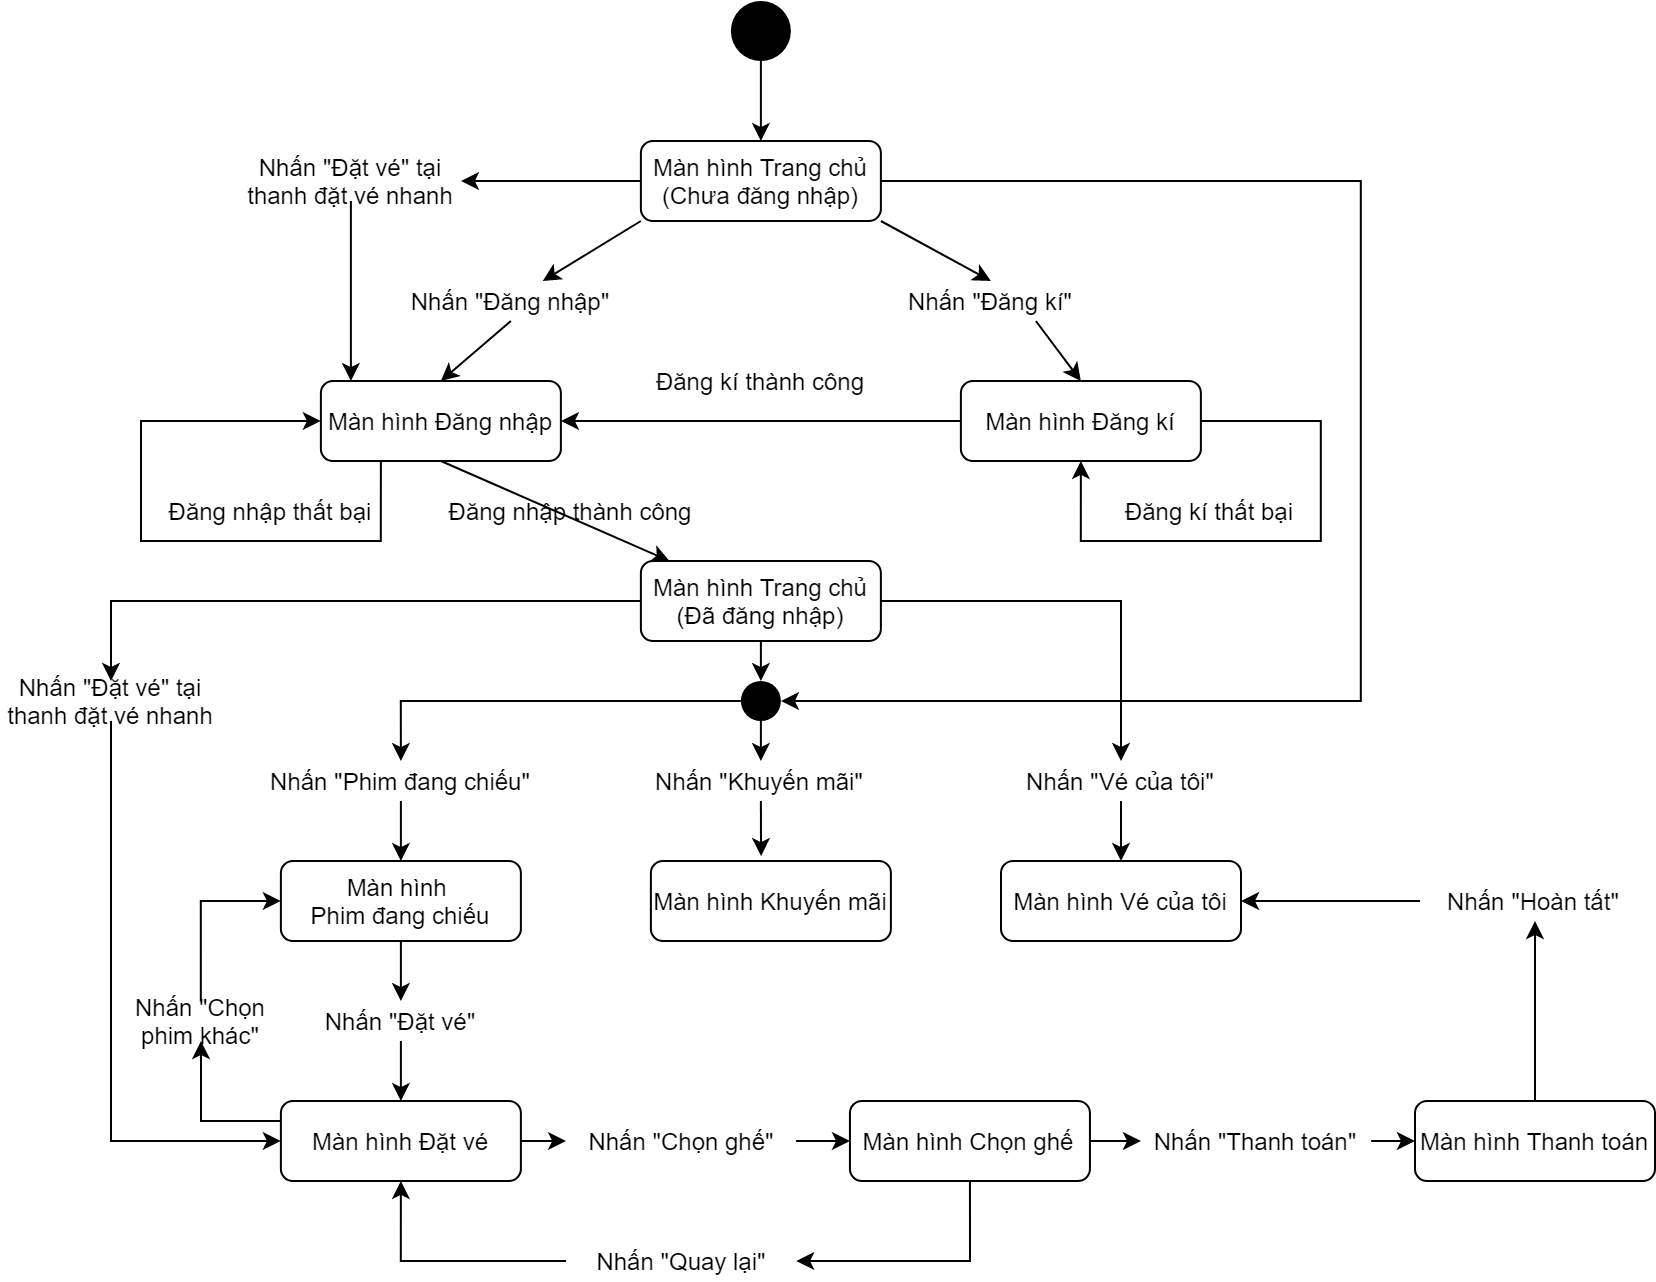
\includegraphics[scale = 0.3]{Diagram/User Screen-flow diagram.png}
						\caption{Sơ đồ điều hướng màn hình người dùng}
					\end{center}
				\end{figure}
			\pagebreak
			\item Bảng mô tả:
				\begin{table}[H]
				\begin{tabular}{|c|c|l|}
				\hline
				STT &
				  Tên màn hình &
				  Ý nghĩa/Ghi chú \\ \hline
				1 &
				  Trang chủ &
				  \begin{tabular}[c]{@{}l@{}}Nơi người dùng sẽ truy cập đầu tiên. Từ đây, người dùng có thể \\ chuyển qua các màn hình Đăng nhập/Đăng kí/Phim đang chiếu\\ /Khuyến mãi/Đặt vé\end{tabular} \\ \hline
				2 &
				  Đăng nhập &
				  \begin{tabular}[c]{@{}l@{}}Nơi người dùng đăng nhập. Sau khi đăng nhập thành công sẽ \\ chuyển về trang chủ\end{tabular} \\ \hline
				3 &
				  Đăng kí &
				  Nơi người dùng đăng kí tài khoản \\ \hline
				4 &
				  Phim đang chiếu &
				  \begin{tabular}[c]{@{}l@{}}Hiển thị danh sách phim đang chiếu và chuyển qua màn hình \\ Đặt vé.\\ Có thể chuyển qua các màn hình khác thông qua navigation bar.\end{tabular} \\ \hline
				5 &
				  Khuyến mãi &
				  \begin{tabular}[c]{@{}l@{}}Hiển thị danh sách khuyến mãi.\\ Có thể chuyển qua các màn hình khác thông qua navigation bar.\end{tabular} \\ \hline
				6 &
				  Vé của tôi &
				  \begin{tabular}[c]{@{}l@{}}Hiển thị danh sách vé đã đặt và giao diện hủy vé.\\ Có thể chuyển qua các màn hình khác thông qua navigation bar.\end{tabular} \\ \hline
				7 &
				  Đặt vé &
				  \begin{tabular}[c]{@{}l@{}}Hiển thị giao diện đặt vé, có thể chuyển qua màn hình Chọn ghế.\\ Có thể chuyển qua các màn hình khác thông qua navigation bar.\end{tabular} \\ \hline
				8 &
				  Chọn ghế &
				  \begin{tabular}[c]{@{}l@{}}Hiển thị giao diện chọn ghế xem phim, có thể chuyển về màn hình\\ Đặt vé, chuyển qua màn hình Thanh toán.\\ Có thể chuyển qua các màn hình khác thông qua navigation bar.\end{tabular} \\ \hline
				9 &
				  Thanh toán &
				  \begin{tabular}[c]{@{}l@{}}Hiển thị thông tin thanh toán, có thể chuyển về màn hình Chọn ghế.\\ Có thể chuyển qua các màn hình khác thông qua navigation bar.\end{tabular} \\ \hline
				\end{tabular}
				\end{table}
		\end{enumerate}

	\subsection{Đặc tả màn hình giao diện}
		\subsubsection{Màn hình 1: Trang chủ}
			\begin{figure}[H]
				\begin{center}
					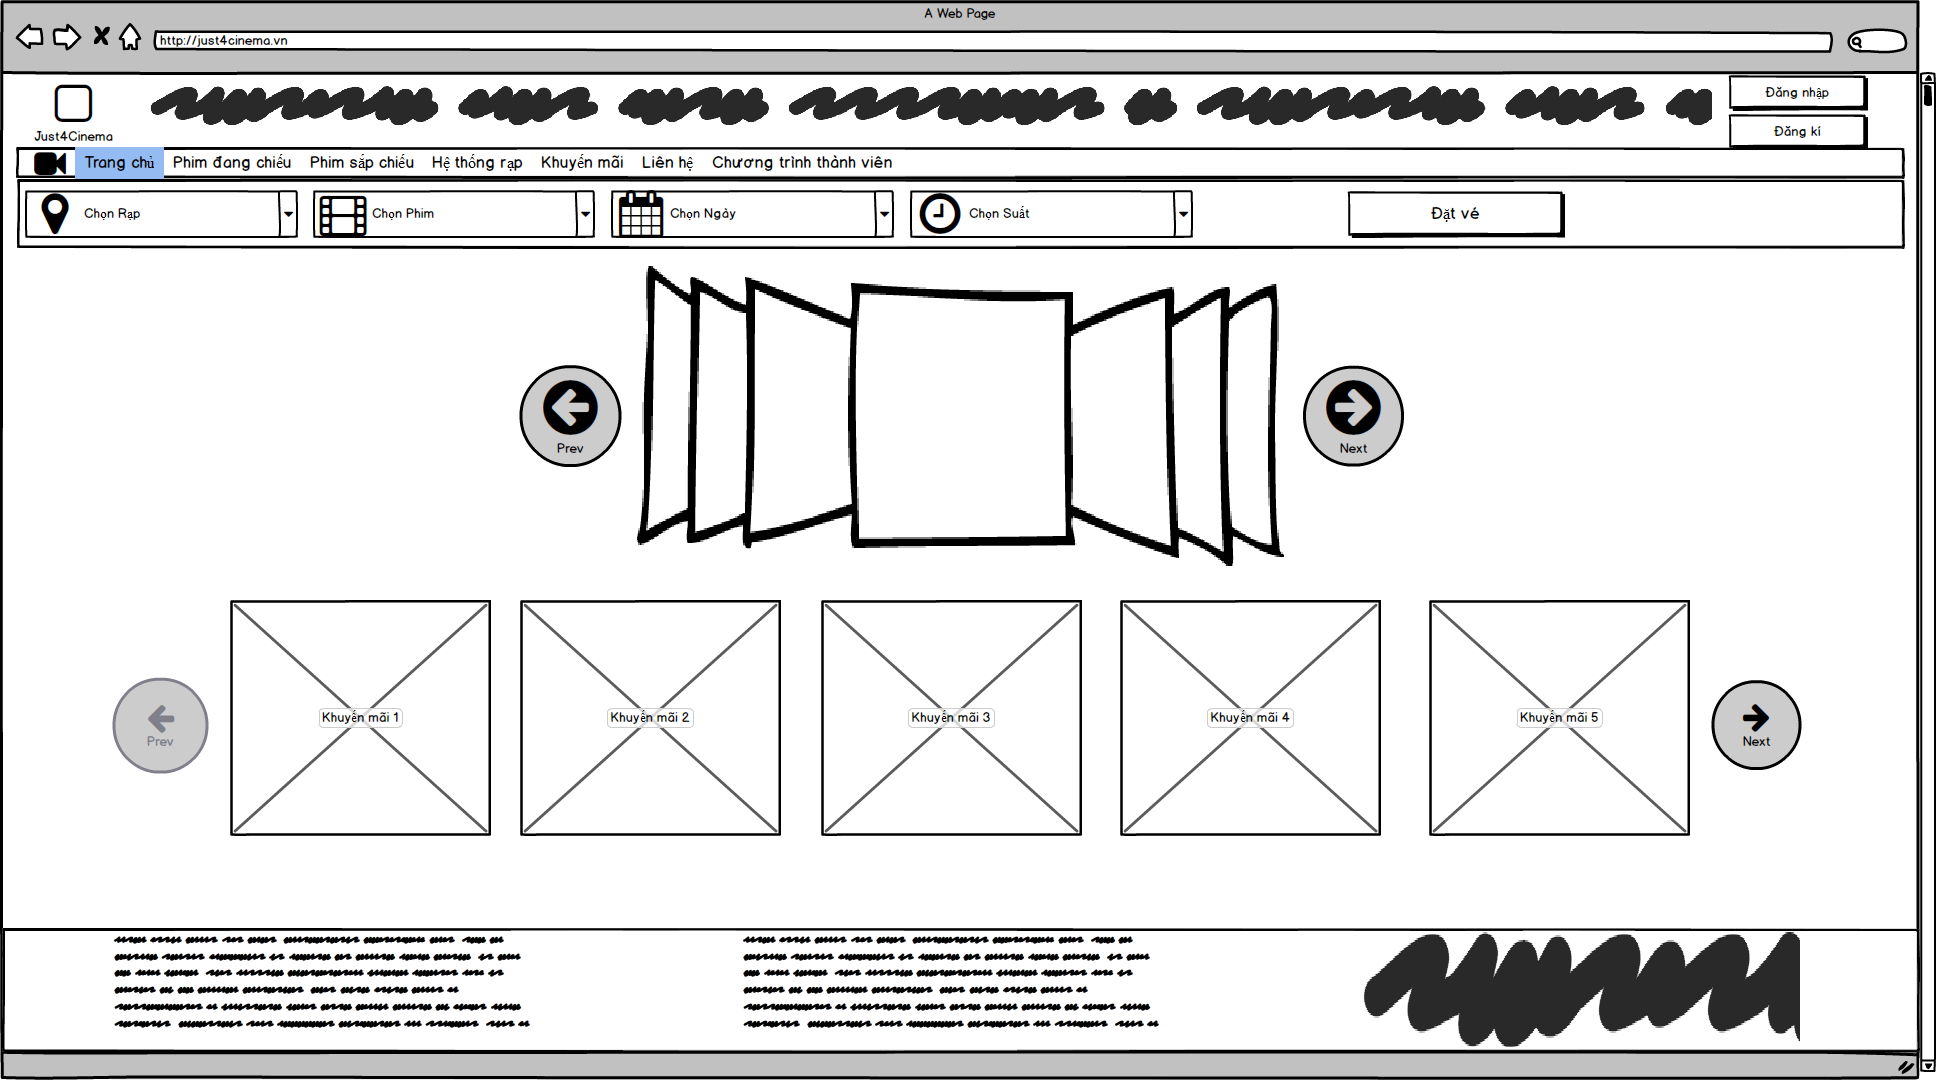
\includegraphics[scale = 0.25]{Wireframe/User/Homepage.png}
					\caption{Màn hình trang chủ}
				\end{center}
			\end{figure}
			Các thành phần chính: 
			\begin{itemize}
				\item Navigation bar
				\item Thanh "Đặt vé" nhanh
				\item Nút "Đăng nhập", "Đăng kí"
				\item Slideshow danh sách các phim đang chiếu, danh sách các khuyến mãi đang có hiệu lực
			\end{itemize}
			Xử lý các event trên màn hình:
			\begin{itemize}
				\item Event click vào các nút trên Navigation bar, nút "Đăng nhập", nút "Đăng kí": Chuyển qua màn hình tương ứng với tên nút
				\item Event click vào nút "Đặt vé" trên thanh đặt vé nhanh: Nếu chưa chọn các thông tin về rạp, phim, suất chiếu thì hiện popup nhắc điền thông tin. Nếu đã chọn đủ các thông tin thì chuyển qua màn hình "Đặt vé"
				\item Event click vào nút mũi tên của slideshow của danh sách phim đang chiếu/khuyến mãi: Chuyển slide theo hướng mũi tên
			\end{itemize}

		\subsubsection{Màn hình 2: Phim đang chiếu/Chọn phim (Trạng thái chưa đăng nhập)}
			\begin{figure}[H]
				\begin{center}
					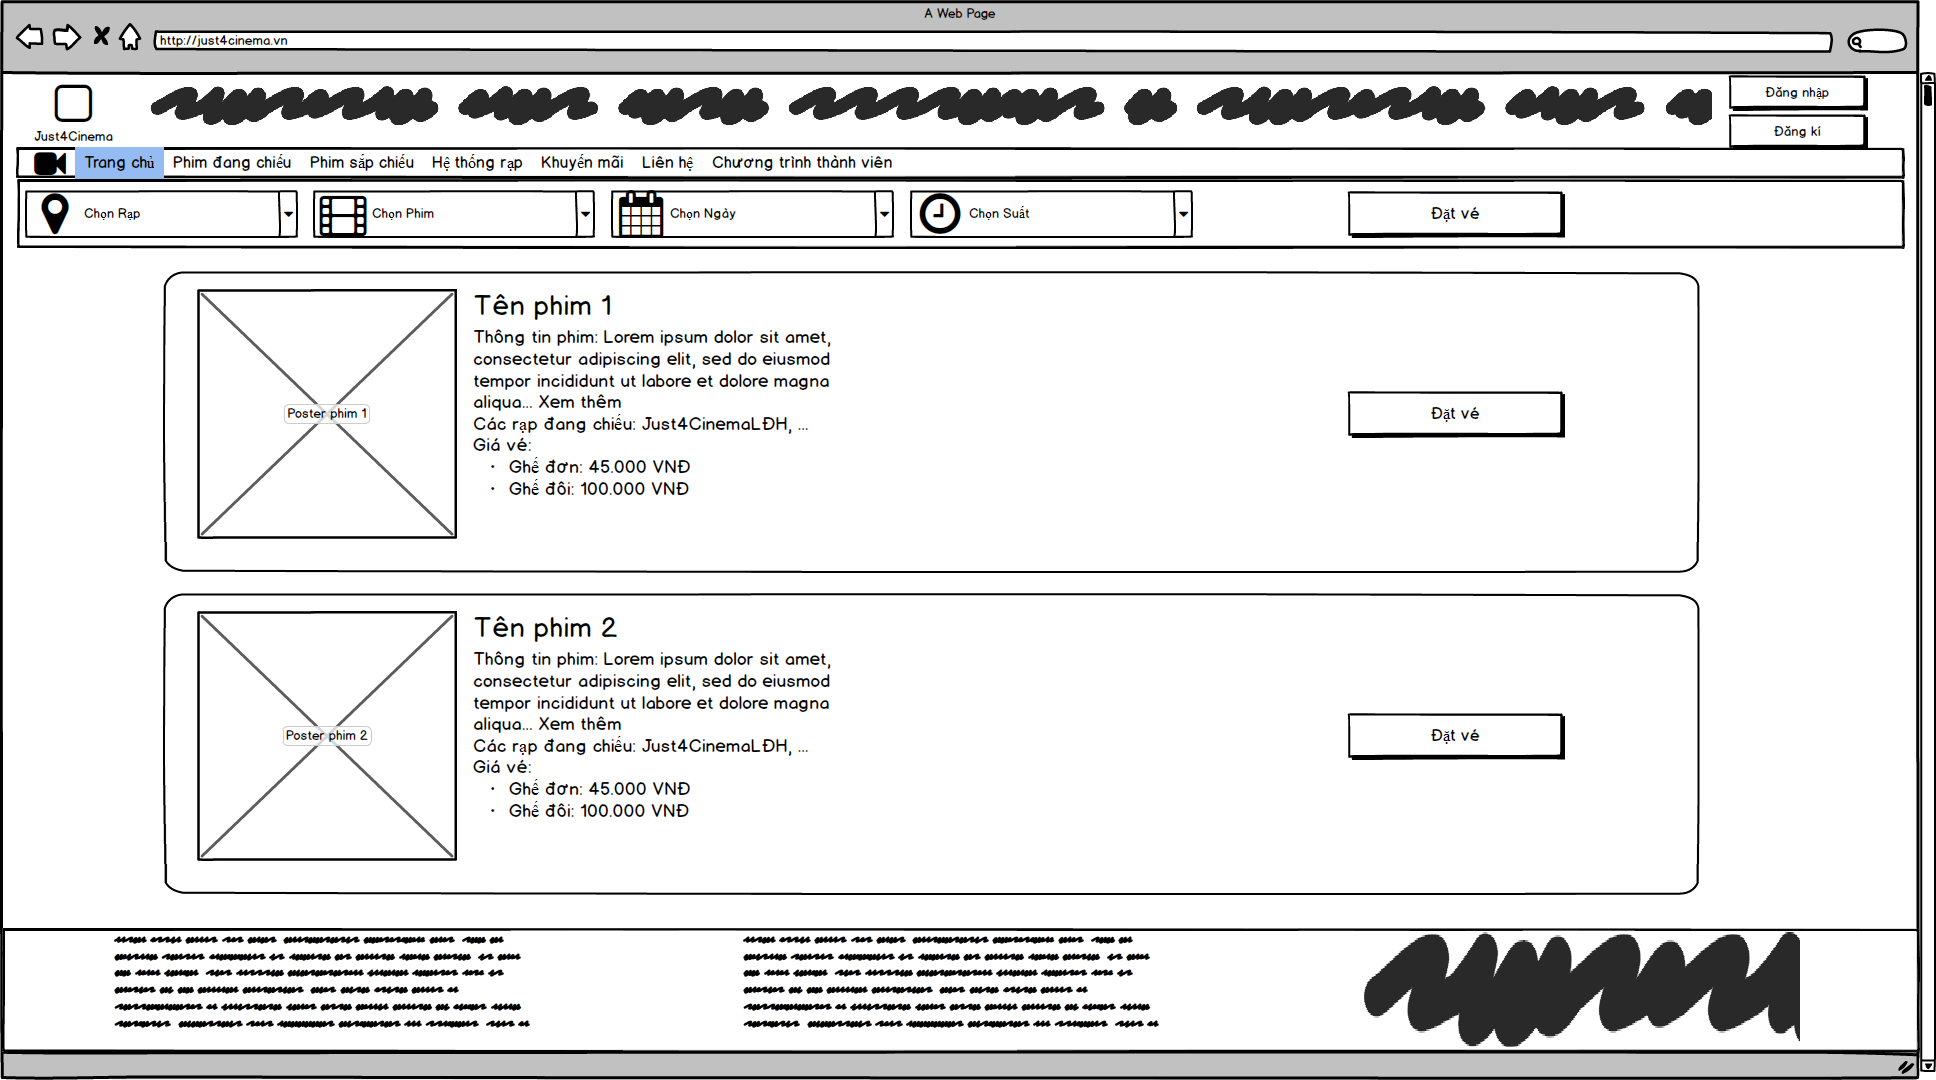
\includegraphics[scale = 0.25]{Wireframe/User/Phim đang chiếu_ Chọn phim.png}
					\caption{Màn hình phim đang chiếu/Chọn phim}
				\end{center}
			\end{figure}
			Các thành phần chính: 
			\begin{itemize}
				\item Navigation bar
				\item Thanh "Đặt vé" nhanh
				\item Nút "Đăng nhập", "Đăng kí"
				\item Danh sách các phim đang chiếu cùng nút "Đặt vé"
			\end{itemize}
			Xử lý các event trên màn hình:
			\begin{itemize}
				\item Event click vào các nút trên Navigation bar, nút "Đăng nhập", nút "Đăng kí": Chuyển qua màn hình tương ứng với tên nút
				\item Event click vào nút "Đặt vé" trên thanh đặt vé nhanh: Nếu chưa chọn các thông tin về rạp, phim, suất chiếu thì hiện popup nhắc điền thông tin. Nếu đã chọn đủ các thông tin thì chuyển qua màn hình "Đặt vé"
				\item Event click vào nút "Đặt vé" trên danh sách phim. Nếu chưa chọn các thông tin về rạp, phim, suất chiếu thì hiện popup nhắc điền thông tin. Nếu đã chọn đủ các thông tin thì chuyển qua màn hình "Đặt vé"
			\end{itemize}

		\subsubsection{Màn hình 3: Đặt vé}
			\begin{figure}[H]
				\begin{center}
					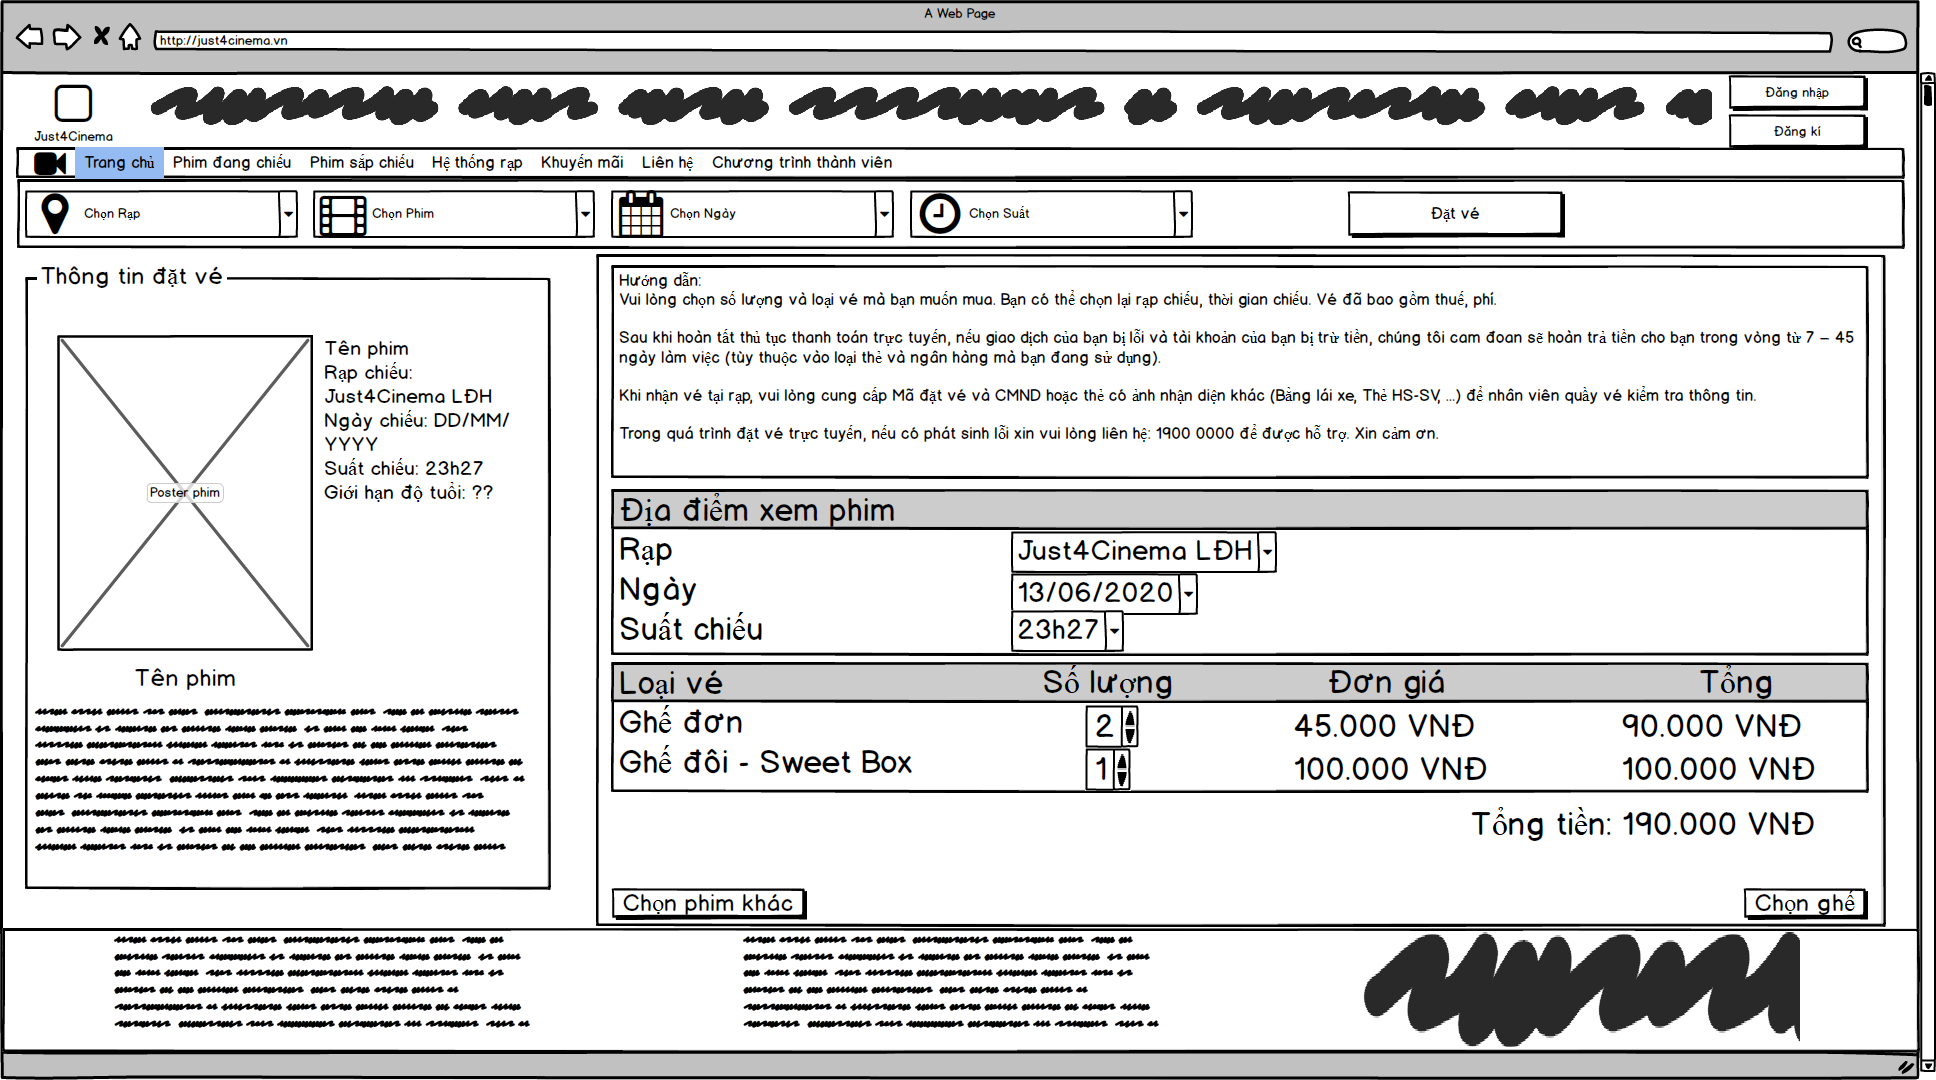
\includegraphics[scale = 0.25]{Wireframe/User/Đặt vé.png}
					\caption{Màn hình Đặt vé}
				\end{center}
			\end{figure}
			Các thành phần chính: 
			\begin{itemize}
				\item Navigation bar
				\item Thanh "Đặt vé" nhanh
				\item Nút "Đăng xuất", "Vé của tôi"
				\item Trường thông tin về vé đang đặt
				\item Các combo box, input field cho phép người dùng chỉnh sửa lại thông tin về rạp, phim, suất chiếu.
			\end{itemize}
			Xử lý các event trên màn hình:
			\begin{itemize}
				\item Event click vào các nút trên Navigation bar, nút "Đăng nhập", nút "Đăng kí": Chuyển qua màn hình tương ứng với tên nút
				\item Event click vào nút "Đặt vé" trên thanh đặt vé nhanh: Nếu chưa chọn các thông tin về rạp, phim, suất chiếu thì hiện popup nhắc điền thông tin. Nếu đã chọn đủ các thông tin thì reload màn hình "Đặt vé" với thông tin mới chọn về rạp, phim, suất chiếu
				\item Event click vào các combo box: Đổ ra thông tin tương ứng với nhãn cho người dùng chọn
				\item Event click vào nút "Chọn ghế": Gửi thông tin vé về server, tạo yêu cầu phát sinh vé, chuyển qua màn hình "Chọn ghế"
				\item Event click vào nút "Chọn phim khác": Chuyển về màn hình "Phim đang chiếu"
			\end{itemize}

		\subsubsection{Màn hình 4: Chọn ghế}
			\begin{figure}[H]
				\begin{center}
					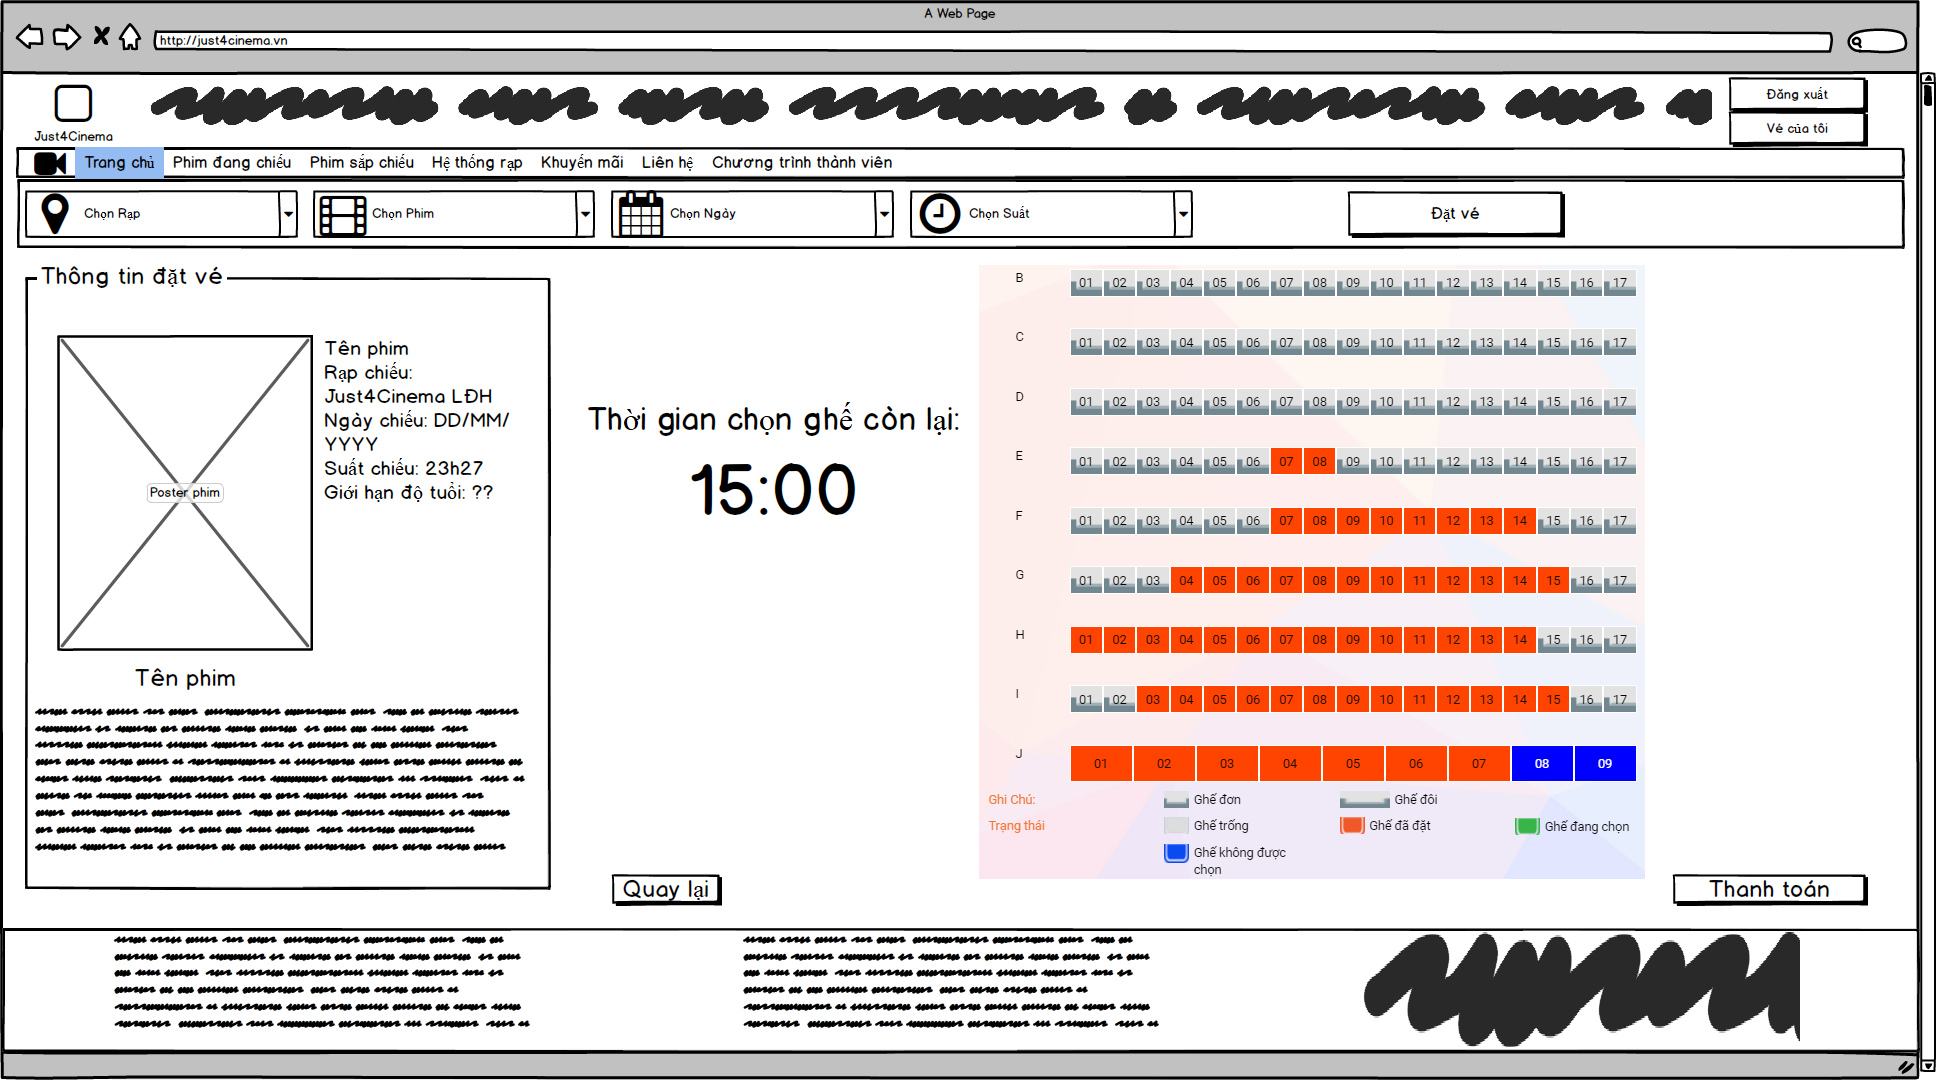
\includegraphics[scale = 0.25]{Wireframe/User/Chọn ghế.png}
					\caption{Màn hình Chọn ghế}
				\end{center}
			\end{figure}
			Các thành phần chính: 
			\begin{itemize}
				\item Navigation bar
				\item Thanh "Đặt vé" nhanh
				\item Nút "Đăng xuất", "Vé của tôi"
				\item Trường thông tin về vé đang đặt
				\item Trường chọn ghế
				\item Đồng hồ chỉ thời gian chọn ghế còn lại
			\end{itemize}
			Xử lý các event trên màn hình:
			\begin{itemize}
				\item Event click vào các nút trên Navigation bar, nút "Đăng nhập", nút "Đăng kí": Chuyển qua màn hình tương ứng với tên nút
				\item Event click vào nút "Đặt vé" trên thanh đặt vé nhanh: Nếu chưa chọn các thông tin về rạp, phim, suất chiếu thì hiện popup nhắc điền thông tin. Nếu đã chọn đủ các thông tin thì chuyển về màn hình "Đặt vé" với thông tin mới chọn về rạp, phim, suất chiếu
				\item Event click vào các icon ghế: Đổi màu icon sang màu xanh lá cây nếu đó là ghế trống - có thể chọn
				\item Event click vào nút "Thanh toán": Gửi thông tin ghế về server, bổ sung mã ghế đã chọnvào thông tin vé, chuyển qua màn hình "Thanh toán"
				\item Event click vào nút "Quay lại": Chuyển về màn hình "Đặt vé"
			\end{itemize}

		\subsubsection{Màn hình 5: Thanh toán}
			\begin{figure}[H]
				\begin{center}
					\includegraphics[scale = 0.25]{Wireframe/User/Thanh toán.png}
					\caption{Màn hình Thanh toán}
				\end{center}
			\end{figure}
			Các thành phần chính: 
			\begin{itemize}
				\item Navigation bar
				\item Thanh "Đặt vé" nhanh
				\item Nút "Đăng xuất", "Vé của tôi"
				\item Trường thông tin về vé đang đặt
				\item Input field của thông tin thanh toán
				\item Trường chính sách và điều khoản thanh toán
			\end{itemize}
			Xử lý các event trên màn hình:
			\begin{itemize}
				\item Load event: Khi màn hình được tải thì phần input field của thông tin thanh toán được điền bởi các thông tin của tài khoản khi đăng kí, có thể thay đổi.
				\item Event click vào các nút trên Navigation bar, nút "Đăng nhập", nút "Đăng kí": Chuyển qua màn hình tương ứng với tên nút
				\item Event click vào nút "Đặt vé" trên thanh đặt vé nhanh: Nếu chưa chọn các thông tin về rạp, phim, suất chiếu thì hiện popup nhắc điền thông tin. Nếu đã chọn đủ các thông tin thì chuyển về màn hình "Đặt vé" với thông tin mới chọn về rạp, phim, suất chiếu
				\item Event click vào các combo box: Đổ ra thông tin tương ứng với nhãn cho người dùng chọn
				\item Event click vào nút "Thanh toán qua Momo": Lưu thông tin thanh toán, gọi API của Momo Service, hỗ trợ thanh toán qua quét mã QR. Reload màn hình với mã QR được sinh ra từ API, yêu cầu người dùng quét để hoàn thành giao dịch.
				\item Event click vào nút "Quay lại": Chuyển về màn hình "Chọn ghế"
			\end{itemize}

\clearpage

\section{Kiểm thử phần mềm}

\subsection{Kế hoạch kiểm thử}

\subsection{Test case}

\subsubsection{Danh sách test case}

\subsubsection{Đặc tả test case}

\clearpage

\section{Quản trị dự án và kế hoạch làm việc}

\subsection{Báo cáo tiến độ}

\begin{itemize}
	\item Các công việc đã hoàn thành
	\begin{itemize}
		\item Xác thực đặt vé, huỷ vé, quản lý thông tin phim phía back-end
		\item Giao diện chức năng đặt vé, huỷ vé
	\end{itemize}
	\item Công việc chưa hoàn thành: Giao diện chức năng quản lý thông tin phim 

	\item Tính tới thời điểm hiện tại, mọi công việc đều đang đi đúng theo tiến độ
	\item Giải pháp làm việc việc đúng tiến độ: Tận dụng thời gian để học công nghệ liên quan đến các công việc cần làm và thực hành nháp để quen với công nghệ mới sau đó bắt tay vào thực hiện công việc
\end{itemize}

\clearpage 

\subsection{Kế hoạch thực hiện}

\begin{itemize}
	\item ID của các tác vụ và các milestone được giải thích chi tiết trong báo cáo 1
	\item Biểu đồ Gantt 
	\begin{figure}[H]
		\begin{center}
			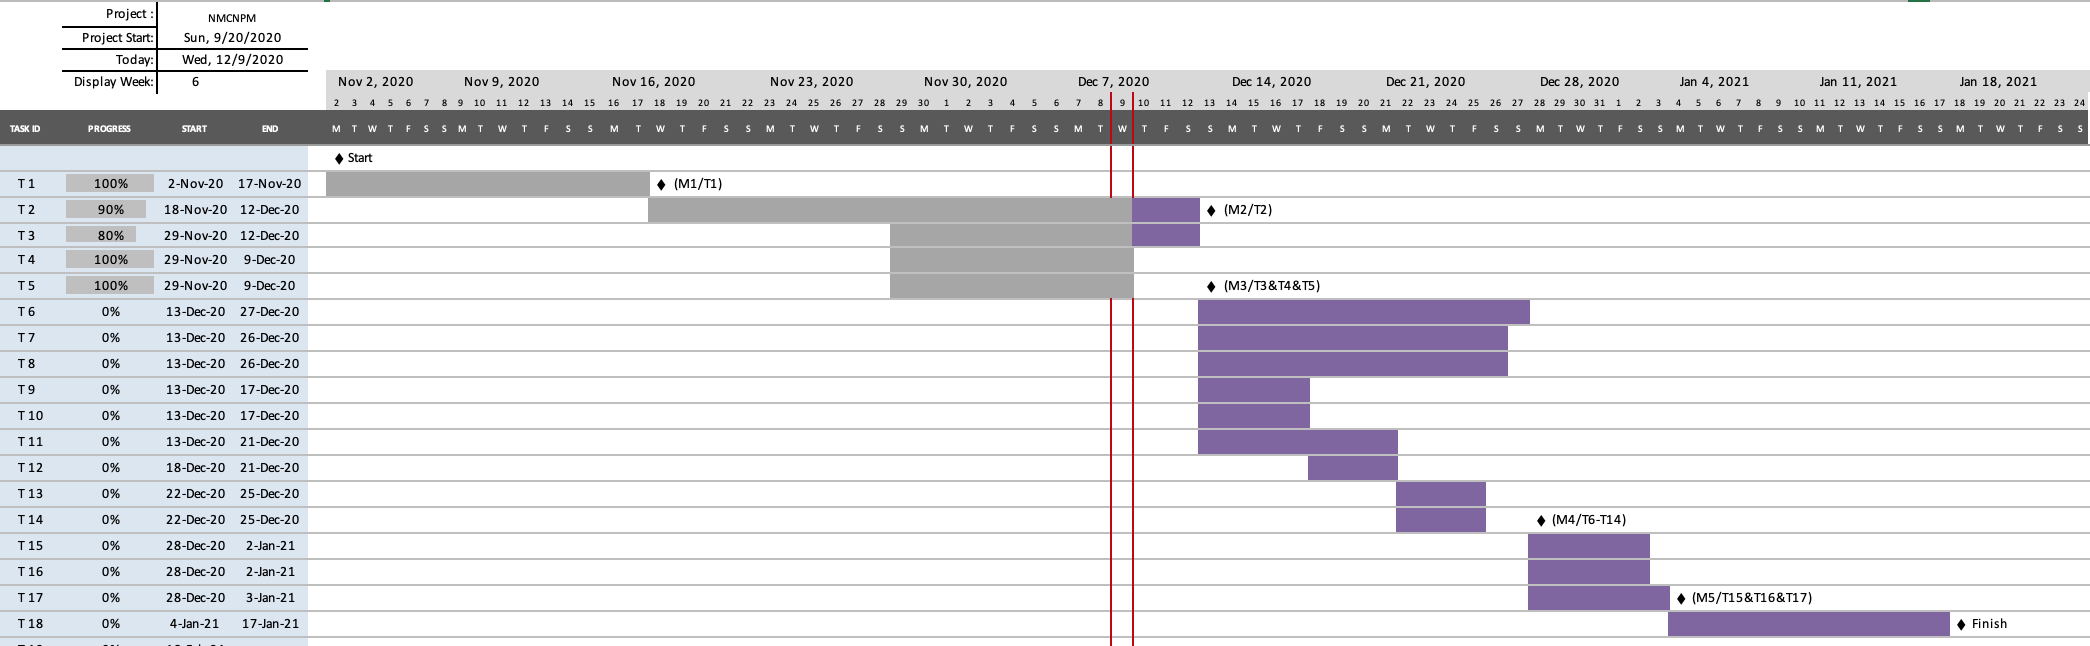
\includegraphics[scale=0.59, angle=90]{./image/gantt.png}
			\caption{Biểu đồ Gantt}
		\end{center}
	\end{figure}
\end{itemize}

\subsection{Phân rã trách nhiệm}

\begin{itemize}
	\item Từ ngày 18/11/2020 đến ngày 12/12/2020, các thành viên trong nhóm chịu trách nhiệm cho các công việc sau
	\begin{table}[H]
		\begin{center}
			\begin{tabular}{|c|l|l|}
			\hline
			STT & \multicolumn{1}{c|}{Họ tên} & \multicolumn{1}{c|}{Công việc}                         \\ \hline
			1 & \multirow{3}{*}{\begin{tabular}[c]{@{}l@{}}- Nguyễn Bảo Long\\ - Phạm Văn Minh Phương\end{tabular}} & Thiết kế giao diện chức năng Huỷ vé    \\ \cline{1-1} \cline{3-3} 
			2   &                             & Thiết kế giao diện chức năng Đặt vé                    \\ \cline{1-1} \cline{3-3} 
			3   &                             & Thiết kế giao diện chức năng Quản lý thông tin phim    \\ \hline
			4 & \multirow{3}{*}{\begin{tabular}[c]{@{}l@{}}- Võ Thế Minh\\ - Phạm Tống Bình Minh\end{tabular}}      & Thiết kế back-end cho chức năng Đặt vé \\ \cline{1-1} \cline{3-3} 
			5   &                             & Thiết kế back-end cho chức năng Huỷ vé                 \\ \cline{1-1} \cline{3-3} 
			6   &                             & Thiết kế back-end cho chức năng Quản lý thông tin phim \\ \hline
			4   & - Nguyễn Duy Vũ             & Triển khai kiểm thử                                    \\ \hline
			\end{tabular}
			\caption{Bảng phân rã trách nhiệm đối với từng công việc cụ thể}
		\end{center}
	\end{table}

	\item Thành viên điều phối việc tích hợp: Phạm Tống Bình Minh 
	\item Thành viên điều phối việc kiểm thử tích hợp: Nguyễn Duy Vũ
\end{itemize}

\clearpage

\section{Tham khảo}

\end{document}